\documentclass[tikz]{standalone}
\usetikzlibrary{calc}
\usepackage{pgfplots}
\usepgfplotslibrary{polar}
\pgfplotsset{compat=1.9}

\begin{document}


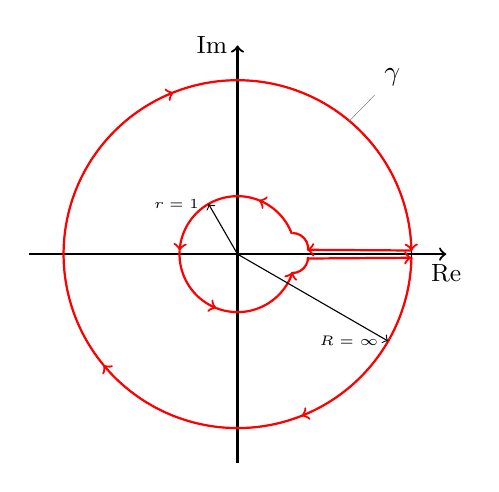
\begin{tikzpicture}[node distance=4cm]
\begin{polaraxis}[
   width=6cm,
   height=6cm,
   clip=false,
   xtick=\empty,
   %xticklabels={$ $, $\frac{\pi}{6}$, $\frac{\pi}{3}$, $ $, $\frac{2\pi}{3}$, $\frac{5\pi}{6}$, $ $, $\frac{7\pi}{6}$, $\frac{4\pi}{3}$, $ $, $\frac{5\pi}{3}$, $\frac{11\pi}{6}$},
   ytick=\empty,
   ymin=0, ymax=3,
   y tick label style={anchor=north east},
   %x coord trafo/.code=\pgfmathparse{#1+40},
   %y coord inv trafo/.code=\pgfmathparse{#1-40},
   %x dir=reverse,
   %xticklabel style={anchor=-\tick-90},
   %yticklabel style={anchor=east, xshift=-4.75cm},
   %y axis line style={yshift=-4.75cm},
   %ytick style={yshift=-4.75cm}
]
\draw[->, thick] (axis cs: 270, 3.6) -- (axis cs: 90, 3.6) node [left] {\small $\mathrm{Im}$};
\draw[->, thick] (axis cs: 180, 3.6) -- (axis cs: 0, 3.6) node [below] {\small $\mathrm{Re}$};

\addplot+[->,thick,domain=0.057:0.19, no markers, red, samples=800] (360*x,1); %
\addplot+[->,thick,domain=0.19:0.49, no markers, red, samples=800] (360*x,1); %
\addplot+[->,thick,domain=0.49:0.69, no markers, red, samples=800] (360*x,1); %
\addplot+[->,thick,domain=0.69:0.95, no markers, red, samples=800] (360*x,1); %
\draw[->, thin] (axis cs: 0, 0) -- (axis cs: 120, 1) node [left] {\tiny $r=1$};

\draw[<-, thick, red] (axis cs: 3.6, 1.2) -- (axis cs: 1.2, 3);
\draw[<-, thick, red] (axis cs: -1.2, 3) -- (axis cs: -3.6, 1.2);

\draw[-, thick, red] (axis cs: 3.6, 1.22) arc [radius=2mm, start angle=-3.6, end angle=90];
\draw[-, thick, red] (axis cs: -19, 1) arc [radius=2mm, start angle=-90, end angle=1];



\addplot+[->,thick,domain=0.003:0.19, no markers, red, samples=800] (-360*x,3); %
\addplot+[->,solid,thick,domain=0.19:0.39, no markers, red, samples=800] (-360*x,3); %
\addplot+[->,solid,thick,domain=0.39:0.69, no markers, red, samples=800] (-360*x,3); %
\addplot+[->,solid,thick,domain=0.69:0.997, no markers, red, samples=800] (-360*x,3); %

\draw[->, thin] (axis cs: 0, 0) -- (axis cs: -30, 3) node [left] {\tiny $R=\infty$};

\node[coordinate, pin=45:{$\gamma$}] at (axis cs: 50, 3) {}; 




%\draw[-, ultra thick] (axis cs: 260, 2) -- (axis cs: 100, 2);

%\node at (axis cs: 200, 0.3) {$-a$};

%\node[circle, fill, pin=-20:{$r$}, inner sep=0.5mm] at (axis cs: 30, 1) {};
\end{polaraxis}
\end{tikzpicture}
\end{document}
